%!TEX program = xelatex
\documentclass[10pt, compress]{beamer}
\usetheme[titleprogressbar]{m}

\usepackage{booktabs}
\usepackage[scale=2]{ccicons}
\usepackage{minted}
\usepackage{comment}
\usepackage{csquotes}
\usepackage[backend=biber,style=authoryear]{biblatex}
\usepackage[main=english]{babel}
\usepackage{amsmath}
\usepackage{amssymb}
\usepackage{amsfonts}
\usepackage{caption}
\usepackage{setspace}
\usepackage{subcaption}
\usepackage{tikz}
\usepackage{pgfplots}
\pgfplotsset{every axis/.append style={very thick}}
\usefonttheme[onlymath]{serif}

\renewcommand*{\nameyeardelim}{\addcomma\space} 
\usepgfplotslibrary{dateplot}
\usemintedstyle{trac}

\setbeamertemplate{section in toc}{\inserttocsectionnumber.~\inserttocsection}
\setbeamercolor{section in toc}{fg=black}

\addbibresource{references.bib}

\title{Distilling explainable semantic textual similarity functions from pretrained transformers}
\date{\today}
\author{Henri Iser \hfill\textit{Supervisor: Eduardo Brito}}
\institute{University of Bonn}


\begin{document}
\maketitle

%\begin{frame}{Gliederung}
%  \tableofcontents
%\end{frame}


%\section{1. Progress Meeting}
\begin{frame}{Sentence Similarity}
\begin{itemize}
	\item \textit{SOTA} model lack explainability
	\item Too slow in some setups
\end{itemize}
\vfill\centering
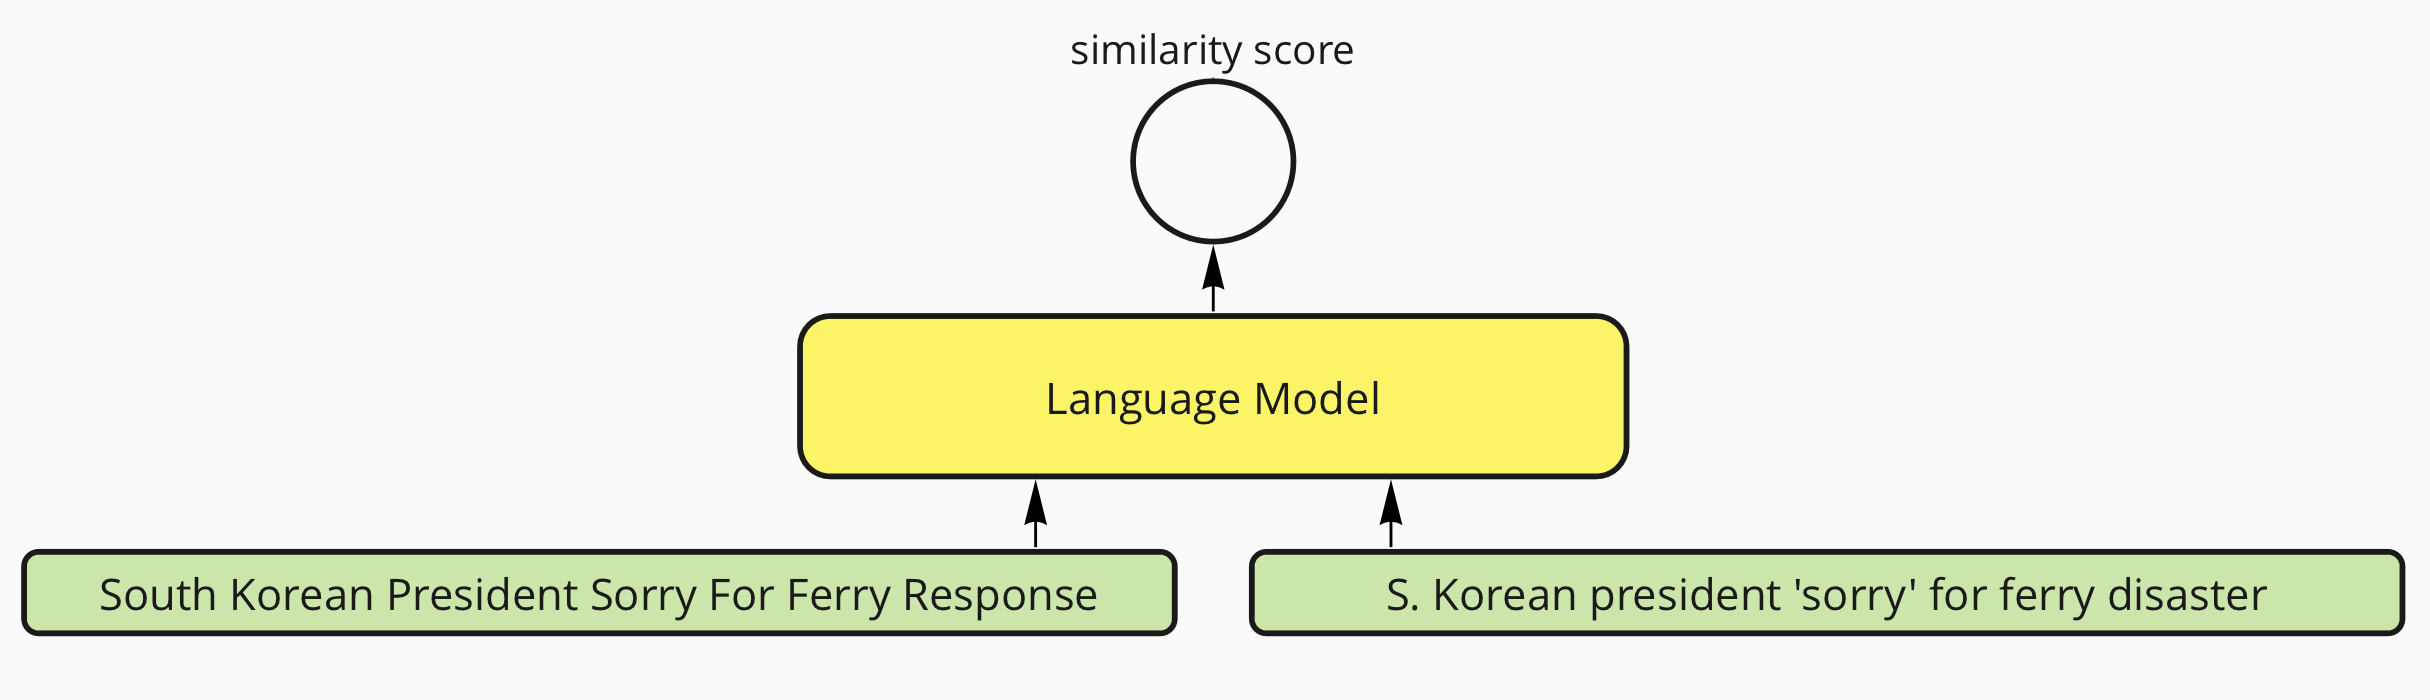
\includegraphics[width=.9\textwidth]{gfx/Similarity}
\end{frame}


\begin{frame}[t]{Explainable Semantic Features}
\begin{itemize}
	\item Topic modeling
	\begin{itemize}
		\item Latent-dirichlet-Allocation (LDA)$^1$
		\item Anchored Correlation Explanation$^2$
	\end{itemize}
\end{itemize}
{\centering
\vfill
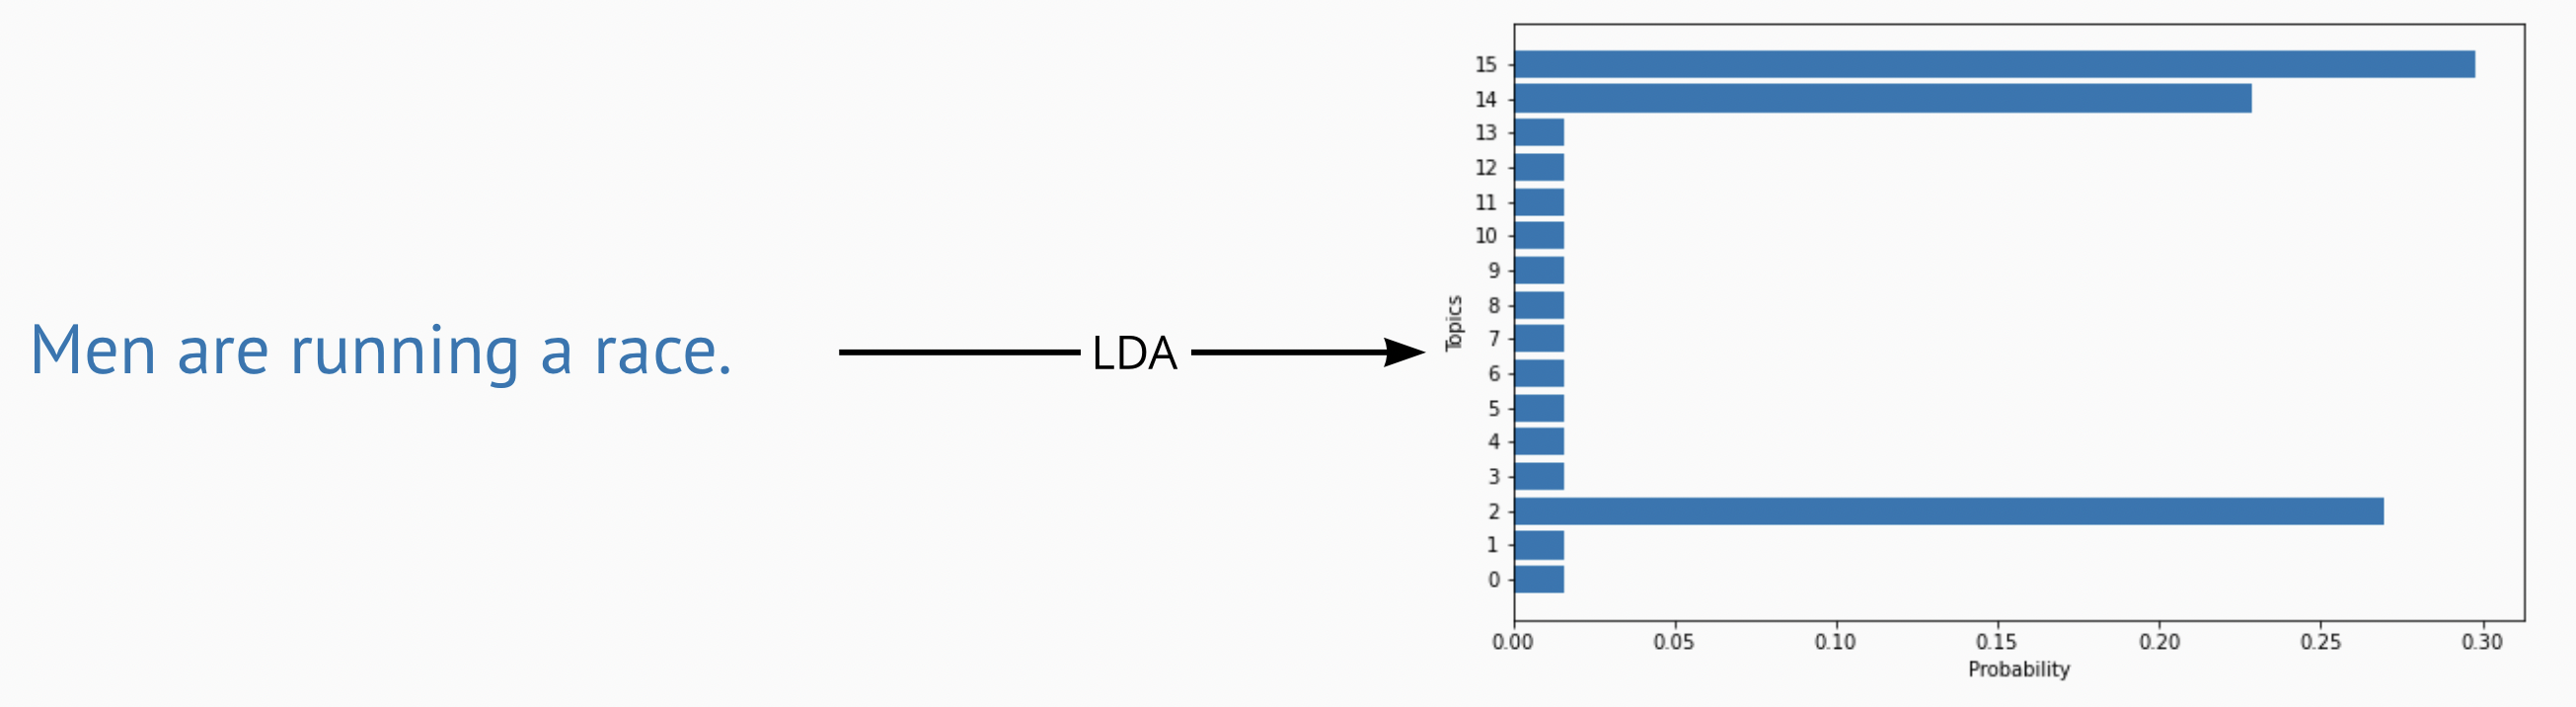
\includegraphics[width=\textwidth]{gfx/LDA}
}
\vfill\vspace{\stretch{100}}
{\setstretch{0}\tiny\raggedright
$^1$ \cite{10.5555/944919.944937}
$^2$ \cite{TACL1244}
}
\end{frame}


\addtocounter{framenumber}{-1}
\begin{frame}[t]{Explainable Semantic Features}
\begin{itemize}
	\item Topic modeling
	\begin{itemize}
		\item Latent-dirichlet-Allocation (LDA)$^1$
		\item Anchored Correlation Explanation$^2$
	\end{itemize}
	\item Part-Of-Speech (POS) tags
\end{itemize}
{\centering
\vfill

\includegraphics[width=\textwidth]{gfx/POS}
}
\vfill\vspace{\stretch{100}}
{\tiny
$^1$ \cite{10.5555/944919.944937}
$^2$ \cite{TACL1244}
}
\end{frame}


\addtocounter{framenumber}{-1}
\begin{frame}[t]{Explainable Semantic Features}
\begin{itemize}
	\item Topic modeling
	\begin{itemize}
		\item Latent-dirichlet-Allocation (LDA)$^1$
		\item Anchored Correlation Explanation$^2$
	\end{itemize}
	\item Part-Of-Speech (POS) tags
	\item Regular Expressions
	\item other ...
\end{itemize}
\vfill\vspace{\stretch{100}}
{\setstretch{0}\tiny\raggedright
$^1$ \cite{10.5555/944919.944937}
$^2$ \cite{TACL1244}
}
\end{frame}


\addtocounter{framenumber}{-1}
\begin{frame}[t]{Explainable Semantic Features}
\begin{itemize}
	\item Topic modeling
	\begin{itemize}
		\item Latent-dirichlet-Allocation (LDA)$^1$
		\item Anchored Correlation Explanation$^2$
	\end{itemize}
	\item Part-Of-Speech (POS) tags
	\item Regular Expressions
	\item other ...
\end{itemize}
\hfill
\textcolor{red}{How to combine these features?}\\
\vfill\vspace{\stretch{100}}
{\setstretch{0}\tiny\raggedright
$^1$ \cite{10.5555/944919.944937}
$^2$ \cite{TACL1244}
}
\end{frame}


\begin{frame}{Framework}
\centering
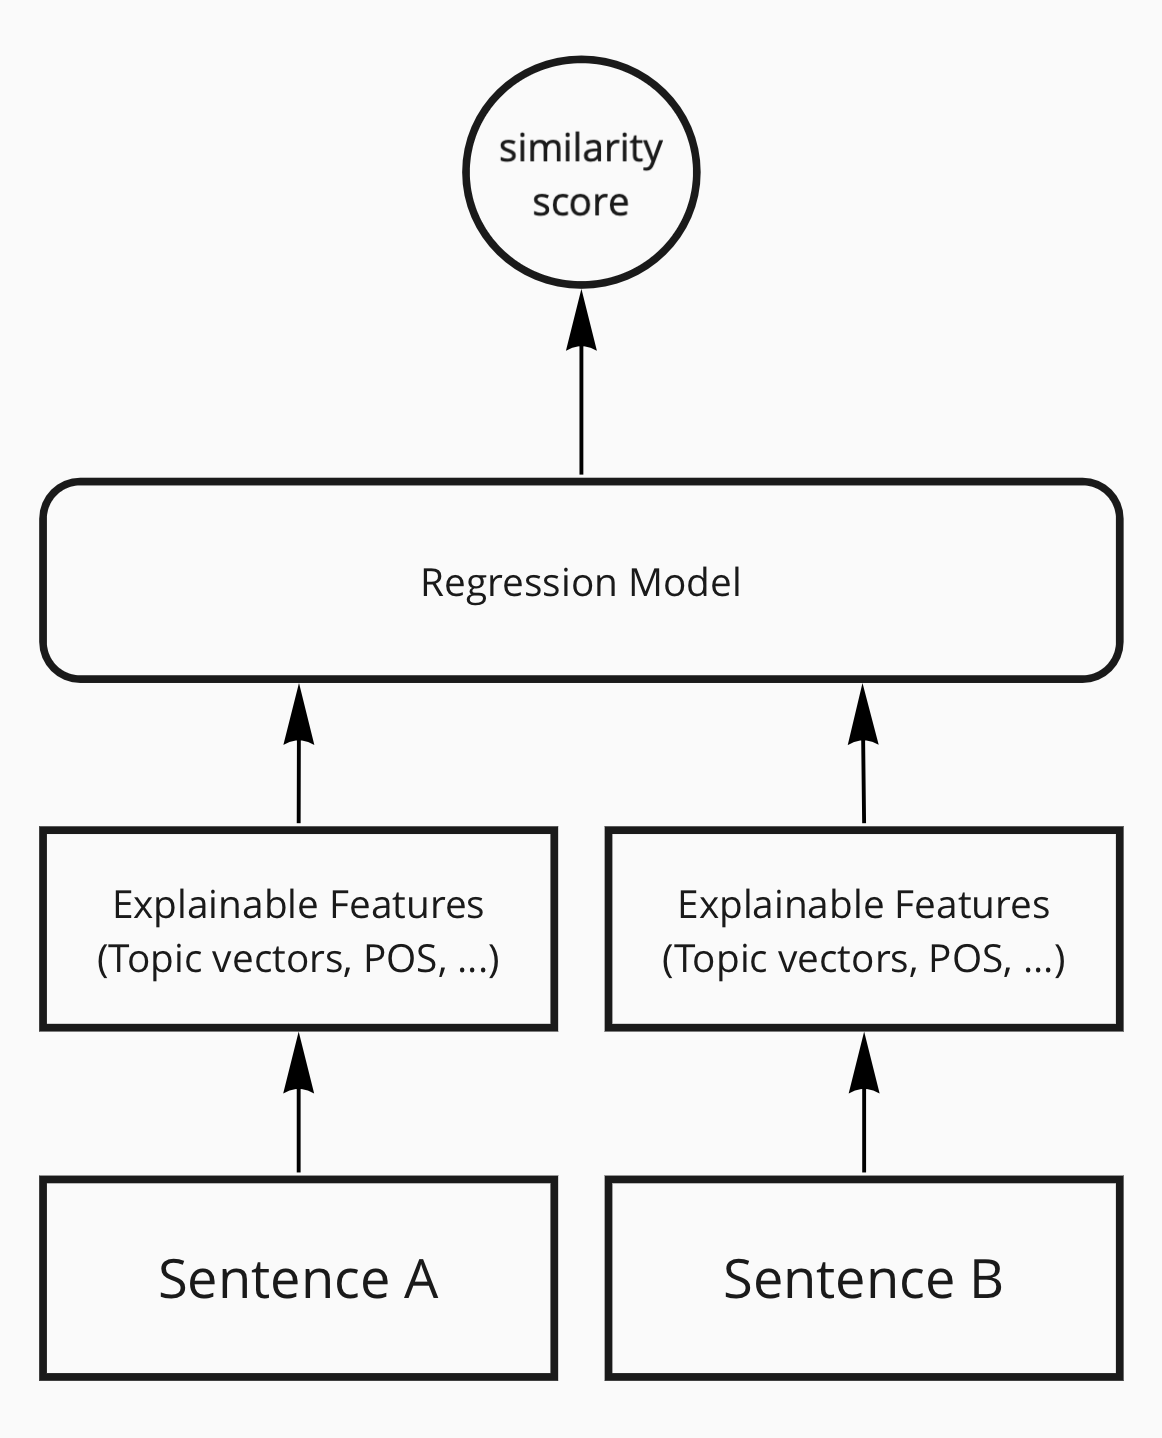
\includegraphics[width=.45\textwidth]{gfx/RegressionModel}
\hfill
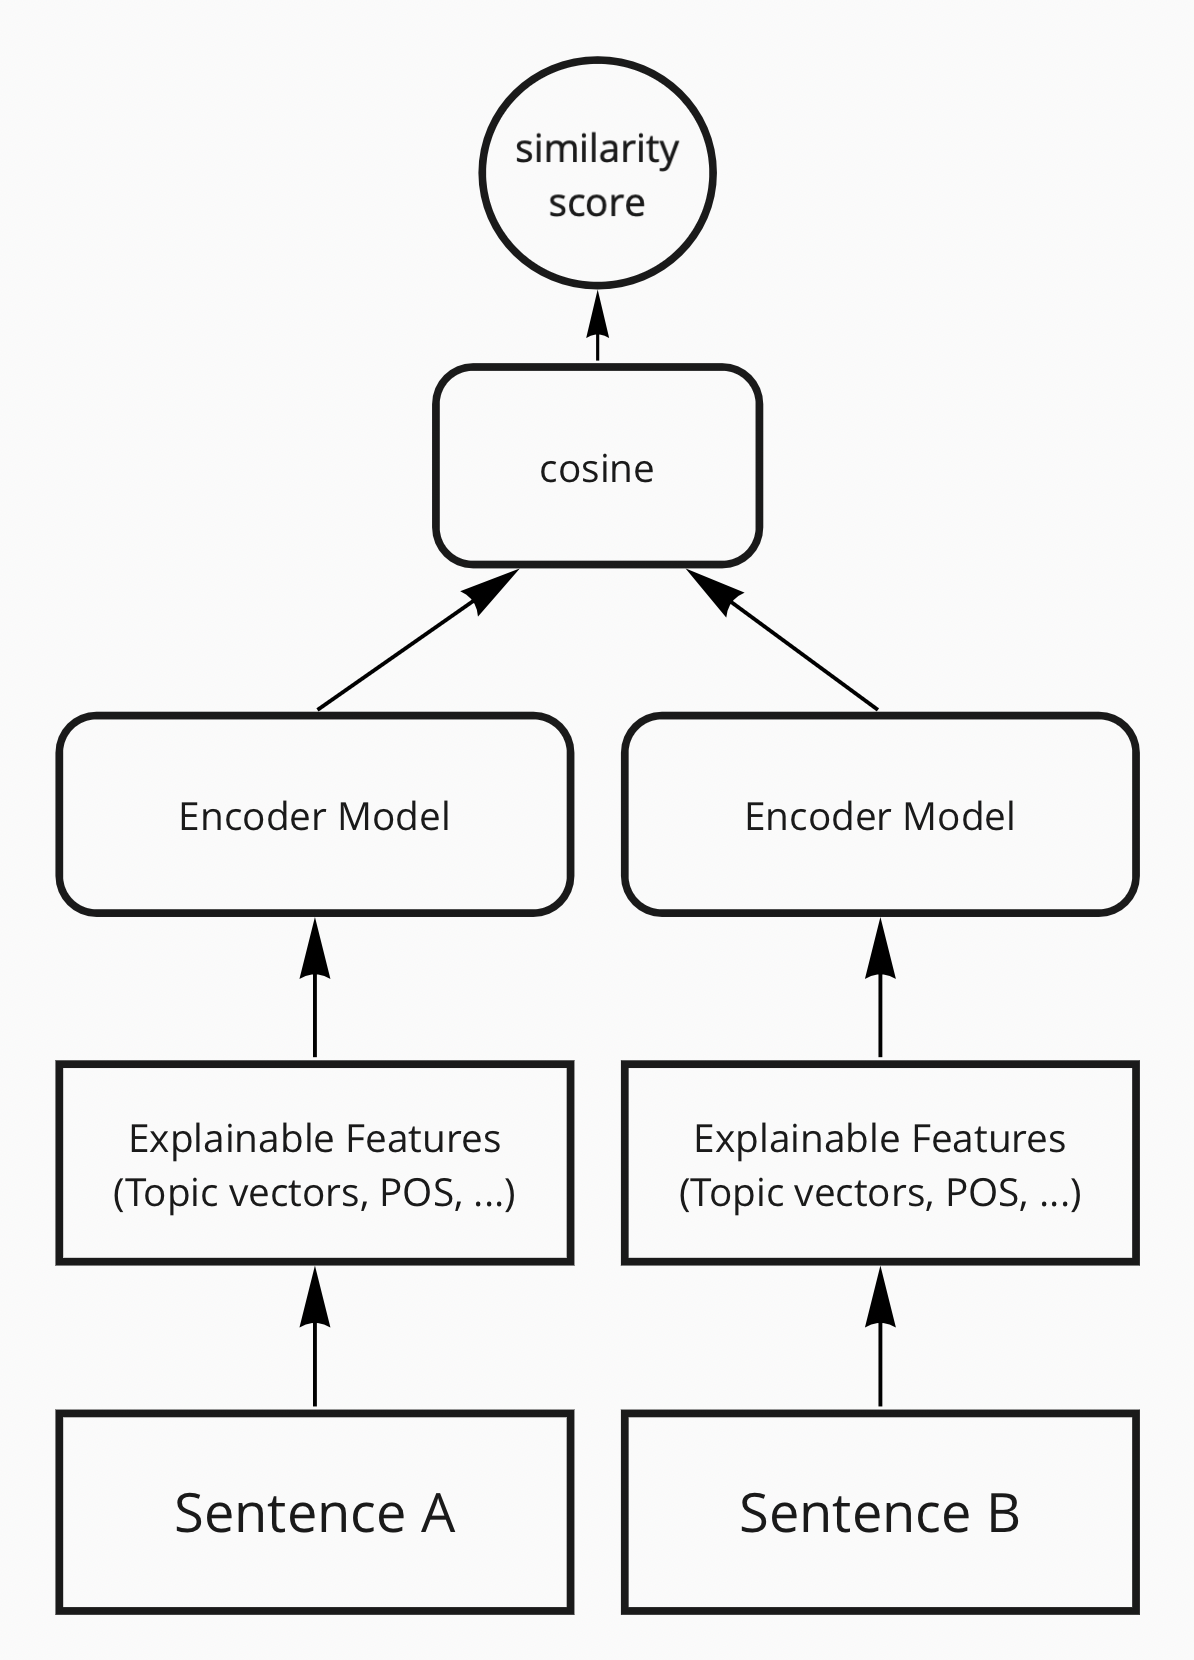
\includegraphics[width=.45\textwidth]{gfx/EncoderModel}
\end{frame}


\begin{frame}{Data}
Datasets:
\begin{itemize}
	\item STS benchmark$^1$
	\item Quora question pairs$^2$
	\item BWS Argument Similarity Corpus$^3$
	\item Microsoft Research Paraphrase Corpus$^4$
\end{itemize}
\vfill\vspace{\stretch{100}}
{\setstretch{0}\tiny
$^1$\url{http://ixa2.si.ehu.eus/stswiki/index.php/STSbenchmark}
$^2$\url{https://quoradata.quora.com/First-Quora-Dataset-Release-Question-Pair}
$^3$\url{https://tudatalib.ulb.tu-darmstadt.de/handle/tudatalib/2496.2}
$^4$\url{https://github.com/wasiahmad/paraphrase_identification}
}
\end{frame}


\begin{frame}{Data Augmentation}
\begin{itemize}
	\item i.e. train set of STS benchmark contains only \#5552 scored sentence pairs.
	\item We need more data to train our model
	\item Use Pre-Trained (Sentence)-BERT Model to create soft labels
\end{itemize}
\vfill
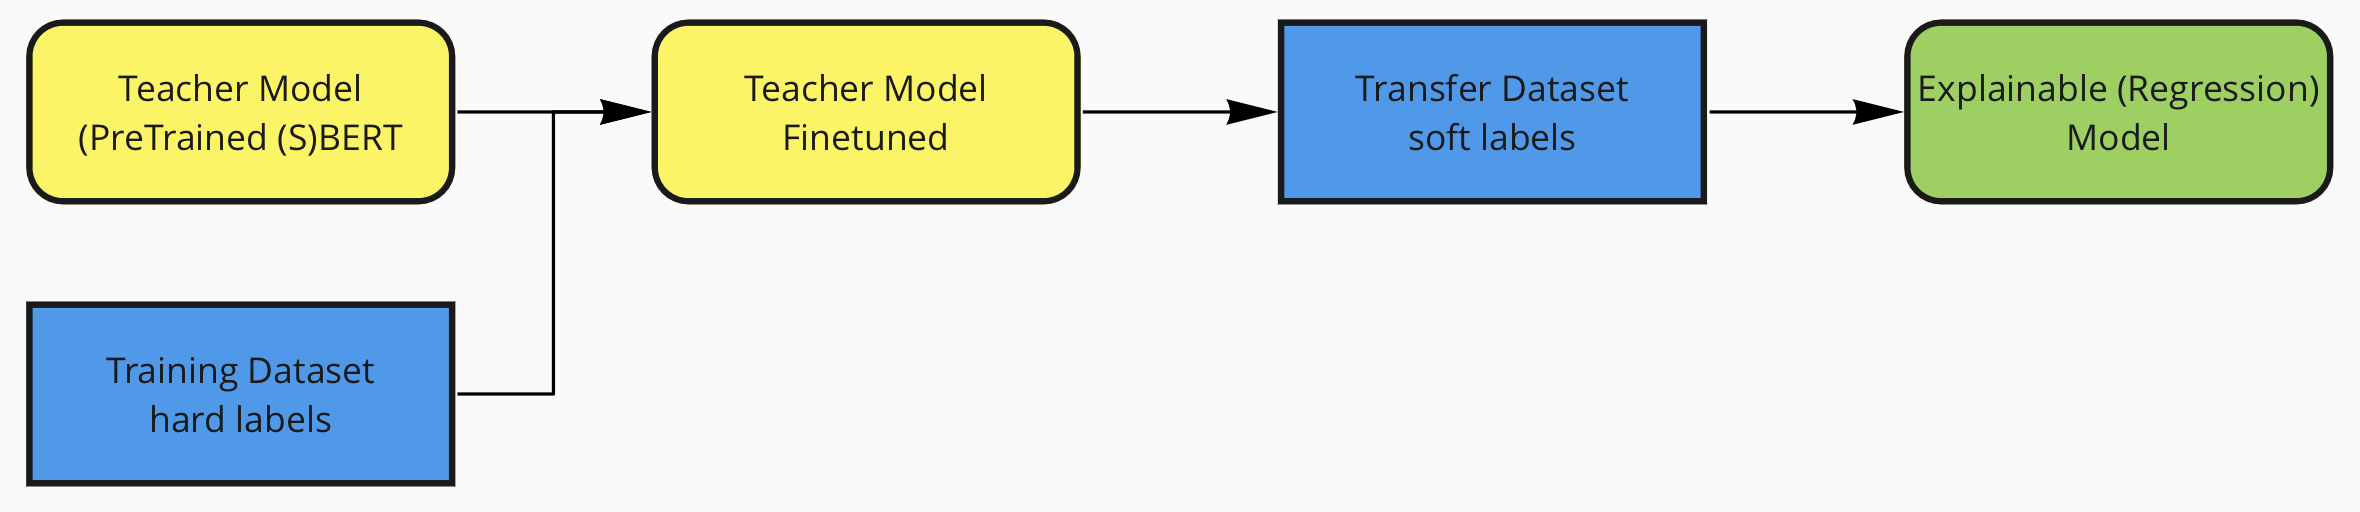
\includegraphics[width=\textwidth]{gfx/DataAugmentation}
\end{frame}


\begin{frame}[t]{Data Augmentation}
Sentence-BERT as Teacher Model
\begin{itemize}
	\item Outperforms \textit{SOTA} sentence embedding methods
	\item High efficiency
	\item Maintains BERT's accuracy
\end{itemize}
\vspace{-1cm}\raggedleft
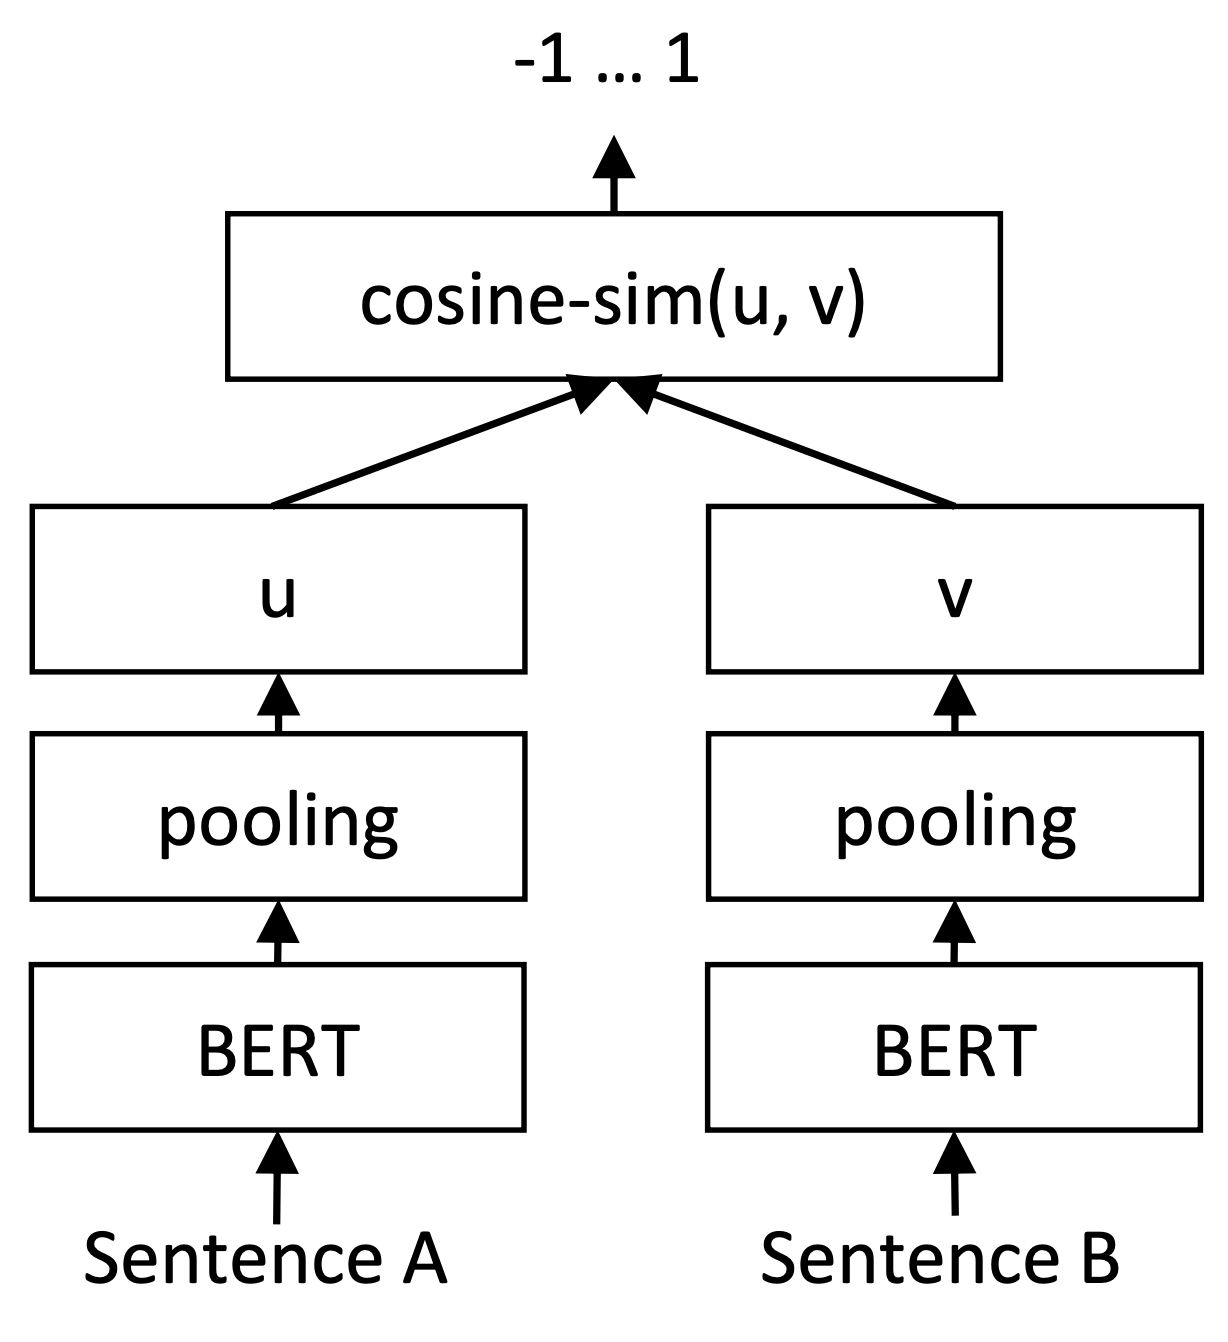
\includegraphics[width=.4\textwidth]{gfx/SBERT}\\
\tiny{\cite{DBLP:journals/corr/abs-1908-10084}}
\end{frame}


\addtocounter{framenumber}{-1}
\begin{frame}[t]{Data Augmentation}
Sentence-BERT as Teacher Model
\begin{itemize}
	\item Outperforms \textit{SOTA} sentence embedding methods
	\item High efficiency
	\item Maintains BERT's accuracy
\end{itemize}
\vspace{-1cm}\raggedleft
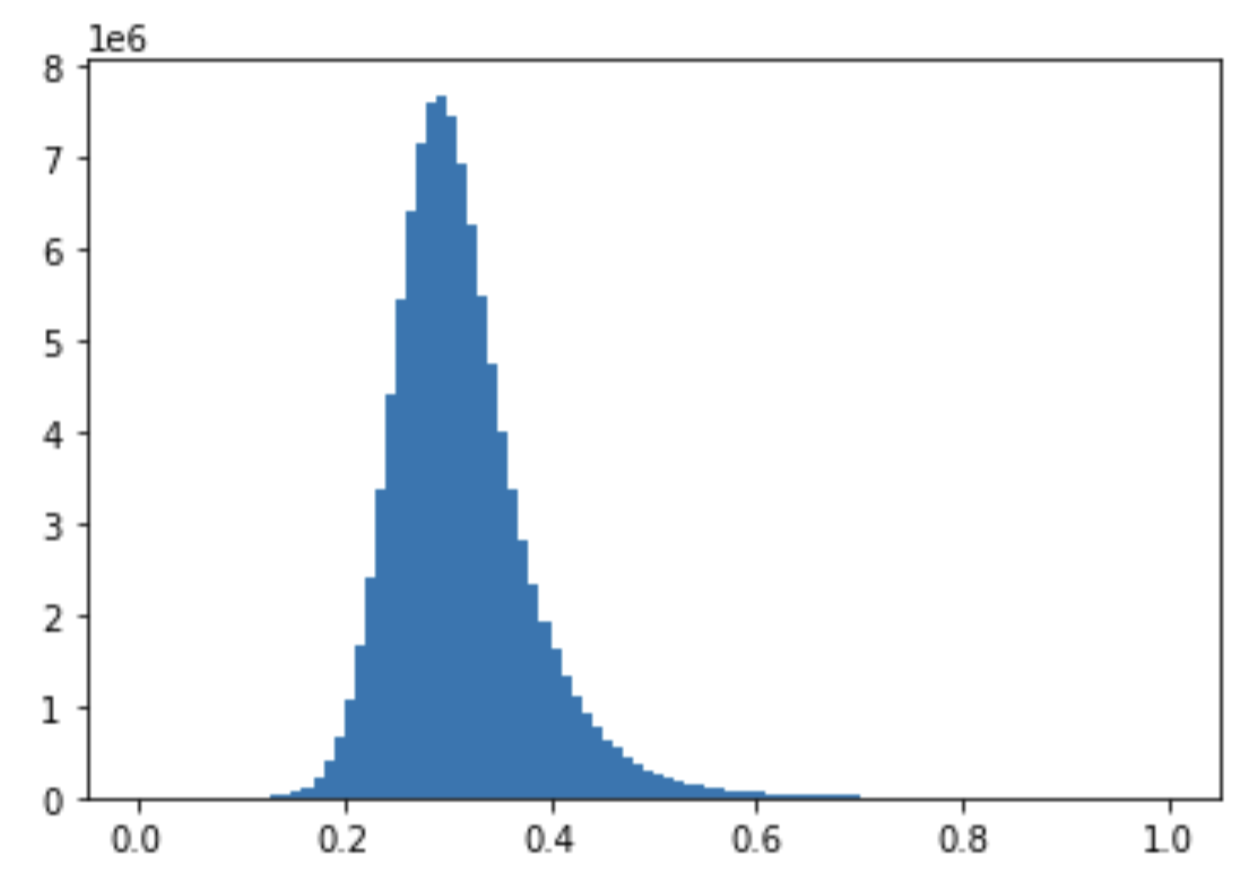
\includegraphics[width=.5\textwidth]{gfx/distribution}
\end{frame}


\begin{frame}{Goals of this Work}
\begin{itemize}
	\item Evaluate similarity scoring task using different semantic features
	\item Compare explainable model against \textit{SOTA}
	\begin{itemize}
		\item Performance
		\item Runtime
	\end{itemize}
	\item Analyse effect of each feature on performance
\end{itemize}
\end{frame}


\begin{frame}{Roadmap}
\hspace*{-1cm}
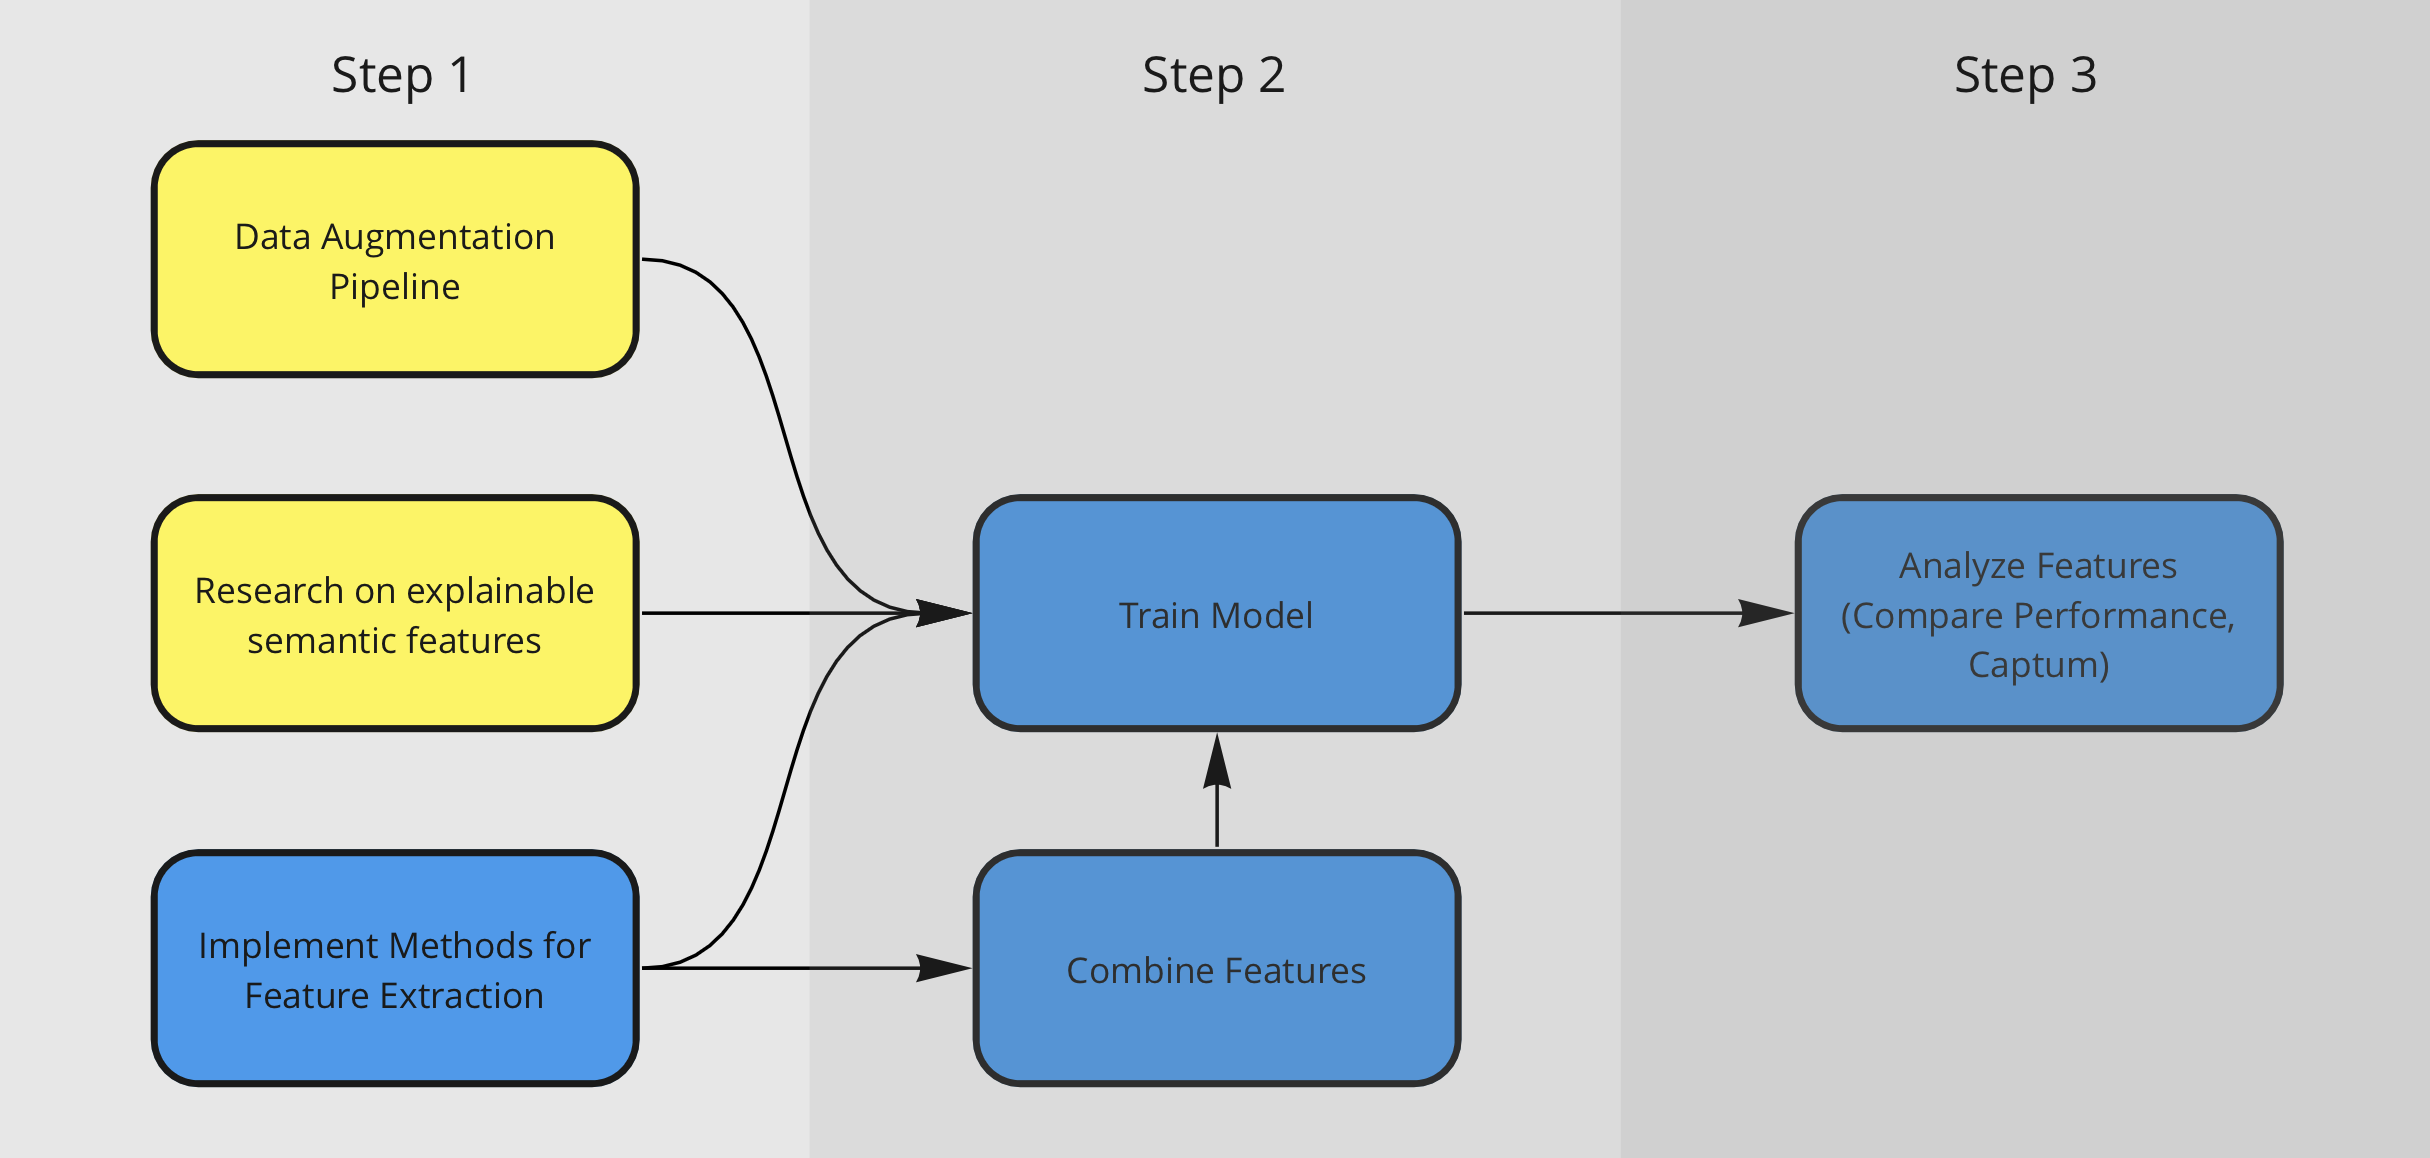
\includegraphics[width=\paperwidth]{gfx/Roadmap}
\end{frame}


\begin{frame}{References}
    \AtNextBibliography{\tiny}
    \printbibliography
\end{frame}

% Begin of workaround: Hide the logo on plain slide
\begingroup
\setbeamertemplate{footline}{}
\plain{Questions?}
\endgroup
% end of workaround

\end{document}
